\chapter{Results}
\label{chap:cpv:results}

The difference in the raw asymmetries of the \pKK\ and \ppipi\ data defines 
\dACP
\begin{equation*}
  \dACP = \ARaw(\pKK) - \ARaw(\ppipi).
\end{equation*}
The values of and uncertainties on \ARaw\ are measured by the weighted fits 
described in \cref{chap:cpv:araw}.
In this section, the combinations of \ARaw\ are made within and across the 
data-taking years (2011 and 2012) and magnet polarities (magnet up and down), 
and the measured values of \ARaw\ and \dACP\ are reported.

\section{Combining measurements}
\label{chap:cpv:results:combination}

The values of \ARaw\ for a given decay mode and data-taking year and polarity 
are measured in the fits.
Within a given year $\zeta$, $\zeta \in [2011, 2012]$, the average value of the 
\ARaw\ for each mode is defined as the arithmetic mean of the two values of 
\ARaw\ measured on the magnet up and magnet down data
\begin{equation}
  \ARaw(\zeta, f) = \frac{%
    \ARaw{}^{\uparrow}(\zeta, f) + \ARaw{}^{\downarrow}(\zeta, f)
  }{%
    2
  }.
  \label{eqn:cpv:results:araw_year}
\end{equation}
The average value of \dACP\ within a year is then defined using the results of 
\cref{eqn:cpv:results:araw_year}
\begin{equation}
  \dACP(\zeta) = \ARaw(\zeta, \pKK) - \ARaw(\zeta, \ppipi).
\end{equation}
Across both years, the values of \ARaw\ are computed as the weighted sum of the 
per-year values, where the weights are the inverses of the squares of the 
statistical uncertainties $\sigma$ on the measurements
\begin{equation}
  \ARaw =
    \frac{1}{\frac{1}{\sigma_{2011}^{2}} + \frac{1}{\sigma_{2012}^{2}}}
    \left(
      \frac{1}{\frac{1}{\sigma_{2011}^{2}}}\ARaw(2011) +
      \frac{1}{\frac{1}{\sigma_{2012}^{2}}}\ARaw(2012)
    \right)
  \label{eqn:cpv:results:araw_polarity}
\end{equation}
This quantity can be computed using the polarity-average \ARaw\ measurements, 
defined in \cref{eqn:cpv:results:araw_year}, and it can also be computed per 
polarity, for example to compute the average magnet down result across 2011 and 
2012.

The measured values of $\ARaw(\pKK)$, $\ARaw(\ppipi)$, and \dACP\ are given in 
\cref{tab:cpv:results:asymmetries}.
Plots of the three measurements for each data sub-sample are given in 
\cref{fig:cpv:results:asymmetries}, where a \chisq\ fit of a constant function 
to the measurements is also shown.
The values are compatible across years and magnet polarities.

The value of \dACP\ averaged across all magnet polarities and years, as 
computed with \cref{eqn:cpv:results:araw_year,eqn:cpv:results:araw_polarity}, 
is measured as
\begin{equation*}
  \dACP = \deltaACP.
  \label{eqn:cpv:results:dacp}
\end{equation*}

\subsection{Unweighted asymmetries}

The results computed without the inclusion of the kinematic weights and phase 
space efficiency corrections are given in 
\cref{tab:cpv:results:asymmetries_unweighted}.
The average value of \dACP\ in these results is measured as
\begin{equation*}
  \dACP = \deltaACPUnweighted.
\end{equation*}
Assuming the weighting does correctly equalise the kinematic, the small change 
in central value from the weighted measurement indicates that the differences 
between the modes before the weighting were small.
The \SI{8}{\percent} reduction in the statistical uncertainty is due to the 
effective increase in the \ppipi\ sample size when unweighted, and illustrates 
that the uncertainty on \dACP\ is dominated by the \pKK\ sample size.

\begin{table}
  \centering
  \caption{%
    Measured asymmetries for each data sub-sample and combination of 
    sub-samples.
    The computation of the combinations, ``2011 + 2012'' and ``Average'', is 
    defined in \cref{chap:cpv:results:combination}.
  }
  \label{tab:cpv:results:asymmetries}
  % \begin{adjustbox}{center}
    \begin{tabular}{ccccc}
  \toprule
  Year & Polarity & \ARaw(\pKK) (\si{\percent}) & \ARaw(\ppipi) (\si{\percent}) & \dACP (\si{\percent}) \\
  \midrule
2011 & Up & $-8.45 \pm 2.29$ & $-11.70 \pm 1.40$ & $3.25 \pm 2.68$ \\
2011 & Down & $-5.82 \pm 1.98$ & $-7.02 \pm 1.16$ & $1.20 \pm 2.29$ \\
2011 & Average & $-7.14 \pm 1.51$ & $-9.36 \pm 0.91$ & $2.22 \pm 1.76$ \\
\midrule
2012 & Up & $-7.52 \pm 1.30$ & $-7.78 \pm 0.83$ & $0.26 \pm 1.54$ \\
2012 & Down & $-7.17 \pm 1.28$ & $-8.49 \pm 0.81$ & $1.32 \pm 1.52$ \\
2012 & Average & $-7.35 \pm 0.91$ & $-8.14 \pm 0.58$ & $0.79 \pm 1.08$ \\
\midrule
$2011 + 2012$ & Up & $-7.75 \pm 1.13$ & $-8.80 \pm 0.72$ & $1.06 \pm 1.33$ \\
$2011 + 2012$ & Down & $-6.77 \pm 1.08$ & $-8.00 \pm 0.67$ & $1.23 \pm 1.27$ \\
$2011 + 2012$ & Average & $-7.29 \pm 0.78$ & $-8.49 \pm 0.49$ & $1.20 \pm 0.92$ \\
  \bottomrule
\end{tabular}
  % \end{adjustbox}
\end{table}

\begin{table}
  \centering
  \caption{%
    Measured asymmetries for each data sub-sample and combination of 
    sub-samples without the inclusion of the kinematic weights and phase space 
    efficiency correction.
    The computation of the combinations, ``2011 + 2012'' and ``Average'', is 
    defined in \cref{chap:cpv:results:combination}.
  }
  \label{tab:cpv:results:asymmetries_unweighted}
  % \begin{adjustbox}{center}
    \begin{tabular}{ccccc}
  \toprule
  Year & Polarity & \ARaw(\pKK) (\si{\percent}) & \ARaw(\ppipi) (\si{\percent}) & \dACP (\si{\percent}) \\
  \midrule
2011 & Up & $-8.73 \pm 2.29$ & $-11.88 \pm 1.05$ & $3.15 \pm 2.53$ \\
2011 & Down & $-5.13 \pm 1.97$ & $-6.24 \pm 0.89$ & $1.10 \pm 2.16$ \\
2011 & Average & $-6.93 \pm 1.51$ & $-9.06 \pm 0.69$ & $2.13 \pm 1.67$ \\
\midrule
2012 & Up & $-7.98 \pm 1.28$ & $-7.78 \pm 0.60$ & $-0.20 \pm 1.41$ \\
2012 & Down & $-6.77 \pm 1.26$ & $-8.94 \pm 0.59$ & $2.17 \pm 1.40$ \\
2012 & Average & $-7.37 \pm 0.89$ & $-8.36 \pm 0.42$ & $0.99 \pm 0.99$ \\
\midrule
$2011 + 2012$ & Up & $-8.16 \pm 1.12$ & $-8.79 \pm 0.52$ & $0.64 \pm 1.24$ \\
$2011 + 2012$ & Down & $-6.29 \pm 1.07$ & $-8.11 \pm 0.49$ & $1.82 \pm 1.17$ \\
$2011 + 2012$ & Average & $-7.26 \pm 0.77$ & $-8.55 \pm 0.36$ & $1.29 \pm 0.85$ \\
  \bottomrule
\end{tabular}
  % \end{adjustbox}
\end{table}

\begin{figure}
  \begin{subfigure}[b]{0.5\textwidth}
    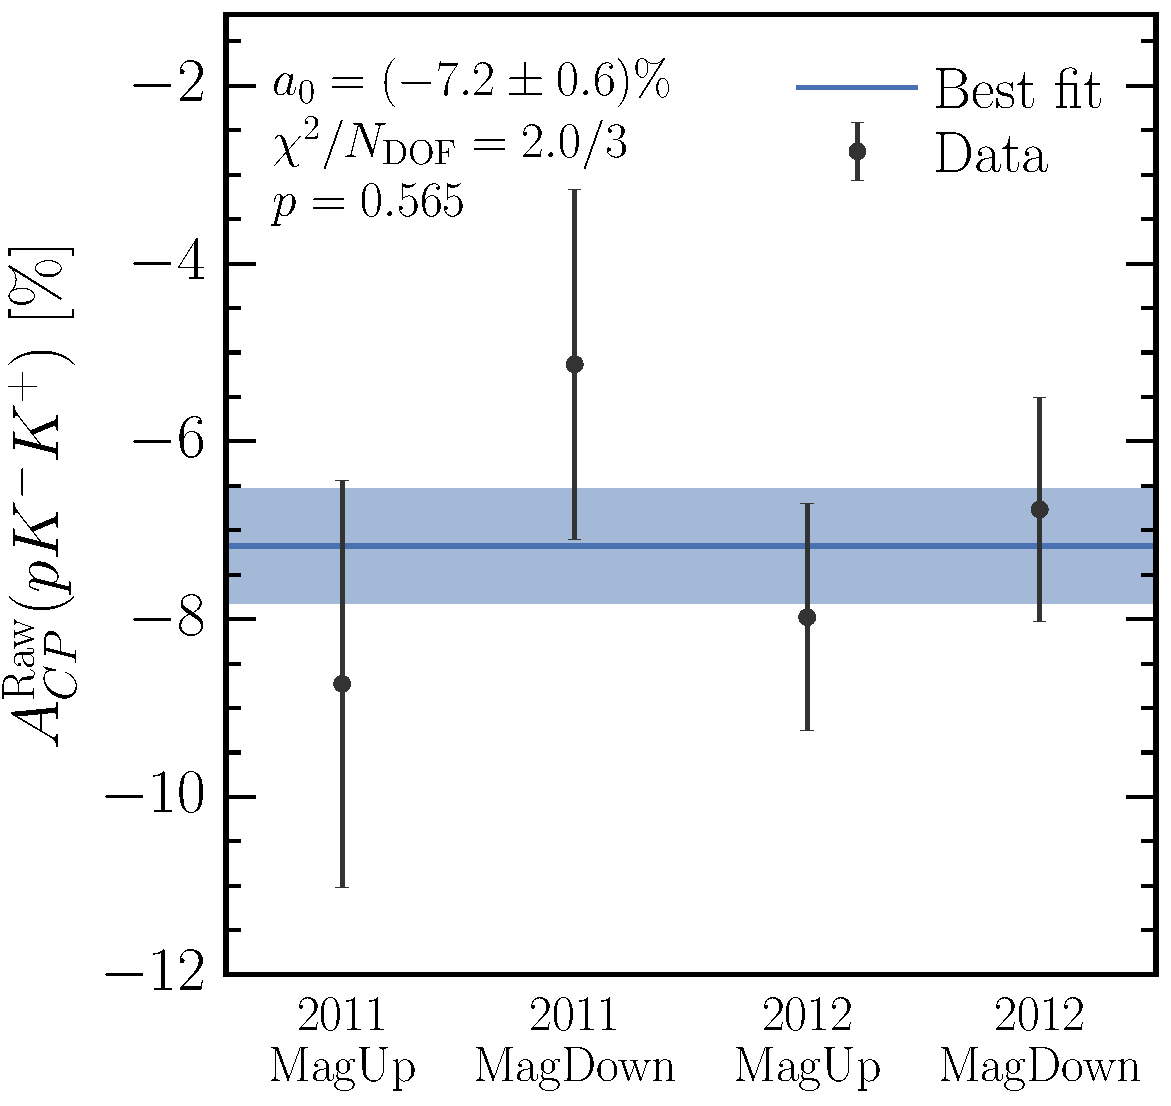
\includegraphics[width=\textwidth]{cpv/results/araw_pKK}
    \caption{$\ARaw(\pKK)$}
    \label{fig:cpv:results:asymmetries:pKK}
  \end{subfigure}
  \begin{subfigure}[b]{0.5\textwidth}
    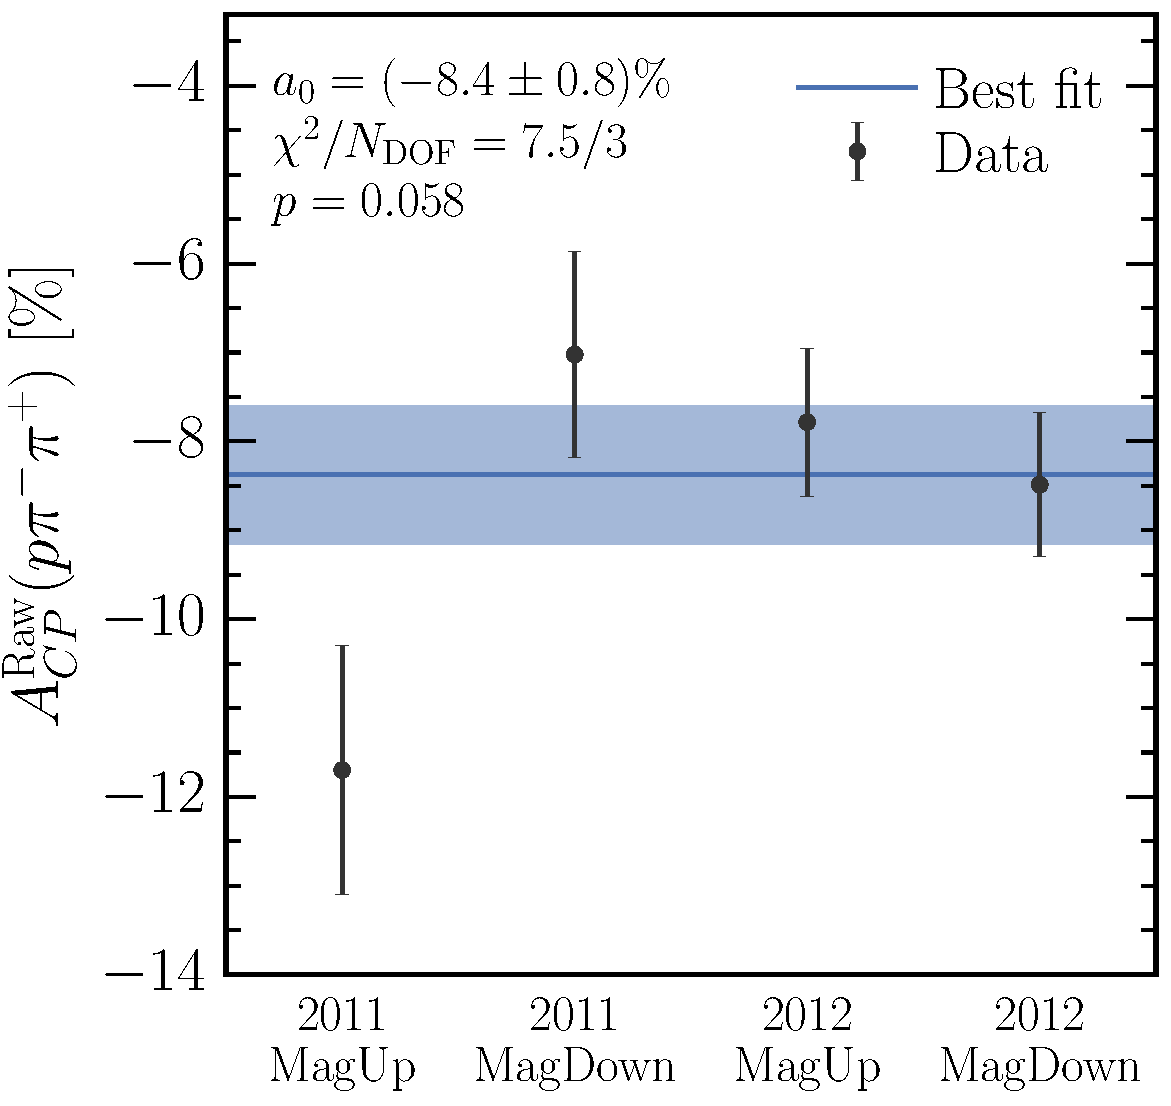
\includegraphics[width=\textwidth]{cpv/results/araw_ppipi}
    \caption{$\ARaw(\ppipi)$}
    \label{fig:cpv:results:asymmetries:ppipi}
  \end{subfigure}

  \vspace{0.5cm}

  \begin{subfigure}[b]{\textwidth}
    \centering
    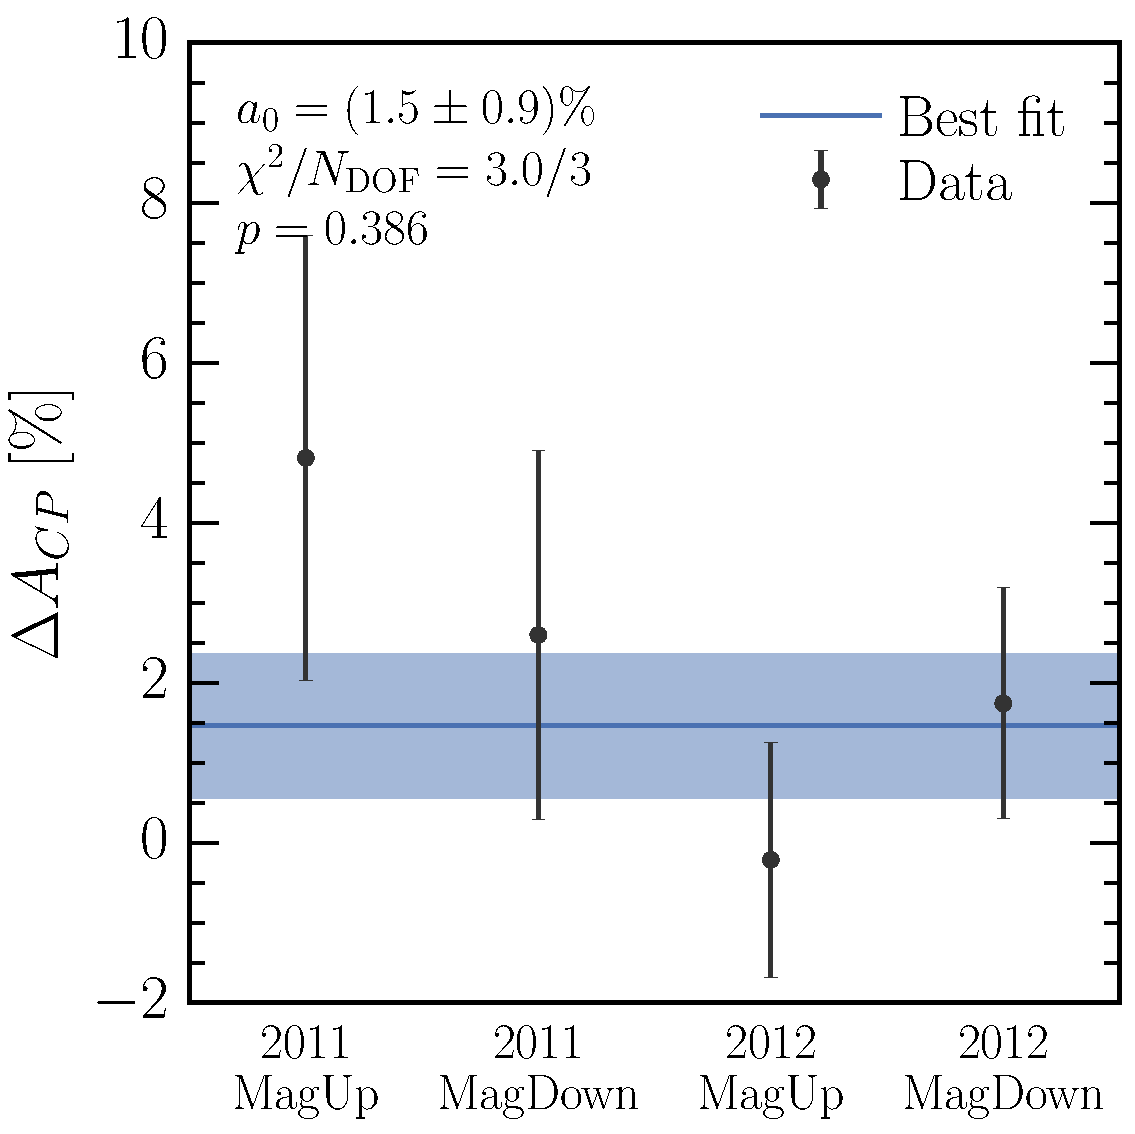
\includegraphics[width=0.5\textwidth]{cpv/results/dacp}
    \caption{\dACP}
    \label{fig:cpv:results:asymmetries:dacp}
  \end{subfigure}
  \caption{%
    Values of the asymmetries $\ARaw(\pKK)$ 
    (\subref*{fig:cpv:results:asymmetries:pKK}), $\ARaw(\ppipi)$ 
    (\subref*{fig:cpv:results:asymmetries:ppipi}), and \dACP\ 
    (\subref*{fig:cpv:results:asymmetries:dacp}), for the four data 
    sub-samples.
    For each asymmetry, a \chisq\ fit of a constant function to the four data 
    points is also shown, along with the best fit value and uncertainty, 
    \chisq\ per degree of freedom~(DOF), and $p$-value.
  }
  \label{fig:cpv:results:asymmetries}
\end{figure}
